% ----------------------------------------------------------
\chapter{Metodologia
}\label{cap:desenvolvimento}
% ----------------------------------------------------------
\section{Interface gráfica}

De forma descritiva, o \textit{Balmy.jl} classifica-se como uma aplicação \textit{web}, isto é, um sistema projetado para utilização através de um navegador, lançando mão de linguagens \gls{HTML}, JavaScript, \gls{CSS} e Julia. Em geral, esse tipo de ferramenta é executada a partir de um servidor \gls{HTTP} ou localmente, no dispositivo do usuário. Na \gls{API} em questão (\textit{Balmy.jl}), a publicação foi feita no GitHub Pages, um servidor gratuito que hospeda sites criados a partir de repositórios Git, um sistema de controle de versionamento distribuído, aplicável principalmente ao desenvolvimento de \textit{software}, pois salva todo o histórico de edições contido no processo de construção de um programa computacional. A função do servidor \textit{web} é receber uma solicitação (requisição) e devolver (resposta) algo para o usuário, mediando essa interação que ocorre em tempo real. 

A infraestrutura da aplicação divide-se em duas partes. A primeira delas é o \textit{front-end}, que corresponde ao \textit{design} gráfico da interface com a qual o usuário lida. Esta é construída com JavaScript, \gls{HTML} e \gls{CSS}, de maneira composta, pois estas são as únicas linguagens de programação que o navegador consegue interpretar. Dentro do contexto, torna-se mandatório preocupar-se com a intuitividade dos elementos adicionados e como a experiência do usuário será delineada dentro da arquitetura da API. Em contrapartida, temos o \textit{back-end}, que dá suporte para a interface e realiza as operações solicitadas sem que o usuário comunique-se diretamente com o código em Julia, linguagem criada especificamente para ciência e mineração de dados, álgebra linear (com a biblioteca nativa chamada \textit{LinearAlgebra.jl}) e aprendizado de máquina. Sua vantagem principal é a velocidade, devido ao fato de ser compilada via tradução dinâmica (\textit{Just In Time}) e por sua tipagem ser forte e dinâmica. Tais fatores contibuem para o incremento significativo no desempenho da linguagem Julia em relação à linguagem Python, por exemplo. No caso dos cálculos que serão realizados, a escolha é justificada porque a linguagem é otimizada para o uso matemático, devido à sua sintaxe adaptada para equações
e expressões numéricas.

As vantagens em desenvolver uma aplicação \textit{web} em relação a um aplicativo \textit{desktop} são muitas, a começar pela total exclusão da necessidade de instalação local (uma vez que a \gls{API} está hospedada em um servidor remoto), que torna-se muito complexa à medida que você adiciona dependências ou muda de sistema operacional. Em razão dessa escalabilidade, todas as atualizações do \textit{Balmy.jl} são/serão realizadas no servidor, ou seja, qualquer alteração na aplicação, já permite o acesso direto a todos os usuários de uma vez só. Como consequência, o custo de manutenção e o tempo de trabalho empregados para incrementar novas funcionalidades ao \textit{site} são reduzidos, pois tudo é feito em um servidor centralizado, sem que o usuário precise atualizar em seu computador pessoal.

Por fim, um último ponto a ser destacado é a usabilidade dos sistemas \textit{web}, que são pensados para oferecer uma experiência diferenciado ao usuário, baseada em múltiplos tipos de dispositivos. Um grande exemplo disso é a responsividade, que consiste em adaptar o conteúdo do sistema à tela do dispositivo utilizado. O endereço eletrônico do \textit{Balmy.jl}, a citar, pode ser acessado tanto por um computador, quanto por um dispositivo móvel (\textit{smartphone}), sendo altamente versátil.

%% vantagens


\section{Representação tridimensional}\label{desenhoestrutural}

As representações tridimensionais das moléculas foram feitas com o \textit{Three.js}, uma biblioteca que usa \textit{WebGL} para renderizar os objetos no espaço. No caso das moléculas, são aplicados modelos conhecidos, como o \textit{ball and stick}), utilizado para exibir geometrias em 3D por meio de bolas (átomos) e bastões (ligações químicas). As esferas são comumente coloridas de acordo com a convenção \gls{CPK}, que se popularizou por distinguir os elementos químicos com um bom contraste. Em 1952, Corey e Pauling publicaram uma descrição dos modelos de preenchimento de espaço de proteínas e outras biomoléculas que eles haviam construído na Caltech \autocite{Corey1953}. Tal proposição foi melhorada em 1965, por Koltun, que estendeu essa técnica aos halogênios e metais \autocite{Crossland2004-ll}. 

Várias das cores do \gls{CPK} referem-se mnemonicamente às cores dos elementos puros ou de seus compostos notáveis. Por exemplo, o hidrogênio é um gás incolor, o carbono como carvão vegetal ou grafite é preto, o enxofre em pó é amarelo, o cloro é um gás esverdeado, o bromo é um líquido vermelho escuro, o iodo no éter é violeta, o fósforo amorfo é vermelho, a ferrugem é vermelho alaranjado escuro, etc. Para algumas cores, tais como as de oxigênio e nitrogênio, a inspiração é menos clara. Talvez o vermelho para o oxigênio seja inspirado no fato de que o químico que contém oxigênio no sangue, hemoglobina, é vermelho vivo; e o azul para o nitrogênio é uma consequência dele ser o principal componente da atmosfera terrestre, que aos olhos humanos parece ser de cor azul (na tonalidade do céu).

Essa convenção foi muito provavelmente inspirada por modelos no século XIX. Em 1865, August Wilhelm von Hofmann, em uma palestra no \textit{Royal Institution} em Londres, estava usando modelos feitos de bolas de \textit{croquet} para ilustrar vários átomos (por exemplo, preto para o carbono, branco para o hidrogênio, verde para o cloro, vermelho para o oxigênio, azul para o nitrogênio)\autocite{Crossland2004-ll}. Na época, o \textit{croquet} era o esporte mais popular na Inglaterra, portanto, as bolas eram abundantes.

Para implementar o modelo molecular utilizando o \textit{Three.js}, é empregado o modelo de Blinn-Phong, capaz de simular superfícies brilhantes com holofotes especulares. O sombreamento é calculado \textit{per pixel} de acordo com o modelo de Phong. Desse modo, apesar de custar um pouco mais de tempo para renderizar, ele atinge uma acurácia maior do que outros modelos disponíveis no \textit{WebGL} (o de Lambert, por exemplo).

No modelo primeiramente proposto por Phong, é calculado continuamente o produto escalar $R \cdot V$ entre um observador $V$ e o feixe de uma fonte de luz ($L$) refletida ($R$) sobre uma superfície. No ajuste proposto por Blinn, no entanto, calcula-se um vetor a meio caminho entre o espectador e os vetores de fonte luminosa, podendo substituir $R \cdot V$ por $N \cdot H$, onde $N$ é o vetor normal à superfície.

\begin{figure}[htb]
\begin{equation}
    \label{eq:R1}
    H = \frac{L + \highlight{blue}{V} }{||L + \tikzmarknode{value}{\highlight{blue}{V}}||}
\end{equation}
\begin{tikzpicture}[overlay,remember picture,>=stealth,nodes={align=left,inner ysep=1pt},<-]
    \path (value.south) ++ (-1,-1.5em) node[anchor=north east,color=blue!67] (scalep){\textit{$V = P_H (-L)$}};
    \draw [color=blue!87](value.south) |- ([xshift=-1.65em,color=blue]scalep.north west);
\end{tikzpicture}
\vspace{2\baselineskip}
\end{figure}

Na \autoref{eq:R1}, $P_H$ é a matriz de Householder que reflete um ponto no hiperplano que contém a origem e tem um vetor normal $H$. Este produto escalar é o cosseno de um ângulo que é metade do ângulo representado pelo produto escalar de Phong (se $V$, $L$, $N$ e $R$ estiverem todos no mesmo plano). Esta relação entre os ângulos sofre desvios discretos quando os vetores não se encontram no mesmo plano, especialmente em relação aos ângulos pequenos.

Ainda sobre os ajustes de Blinn ao modelo de Phong, consideremos que o ângulo entre o vetor a meio caminho $(N \cdot H)$ e a superfície normal é provavelmente menor do que o ângulo entre $R$ e $V$ usado no modelo original (a menos que a superfície seja vista de um ângulo muito íngreme para o qual é provável que seja maior), e já que Phong está usando $(R \cdot V)^\alpha$, um expoente (chamado de constante de brilho) pode ser definido como $\alpha' > \alpha$, tal que $(N \cdot H)^{\alpha'}$ está mais próxima da expressão original de Phong. Os resultados das estruturas geradas no \textit{Balmy.jl} estão na \autoref{design}.

Para detectar as ligações químicas, foi implementado um algoritmo baseado nos raios covalentes de van der Waals, que representa, pictoricamente, o raio de uma esfera sólida imaginária empregada para representar um átomo. Tal parâmetro é representado a partir de definições termodinâmicas da equação de estado de van der Waals, onde $N_a$ é o número de Avogadro e $r$ é o raio.

\begin{equation}
    b = \frac{16}{3} \pi N_a r^3
\end{equation}

Os parâmetros $a$ e $b$ são obtidos experimentalmente e dependem da natureza do gás. O fator de correção $b$ é denominado volume de exclusão, referindo-se tanto ao volume próprio dos átomos, como o volume circundante onde não pode haver outros porque nessa distância predominam as forças de repulsão entre os átomos do gás (forças de van der Waals). Desse modo, se a distância entre os dois átomos que estão sendo analisados é maior do que a soma dos seus raios de van der Waals, não é detectada uma ligação química pelo \textit{Balmy.jl}.

\section{Método de Hueckel Estendido}

O \gls{HMO} foi inicialmente proposto por Erich Hueckel em 1930 \autocite{Hckel1931} como uma alternativa para calcular orbitais moleculares como combinações lineares de orbitais atômicos\autocite{Coulson1978-ot}. Tal teoria prediz os orbitais moleculares de elétrons $\pi$ em moléculas com estrutura eletrônica deslocalizada., tal como o etileno, benzeno, butadieno e piridina. Isso nos fornece uma base teórica para fundamentar a regra de Hueckel, responsável por enunciar que moléculas cíclicas, planares ou espécies químicas iônicas com $4n + 2$ elétrons $\pi$ são aromáticos, sendo $n$ um número inteiro positivo $0, 1, 2, \cdots, n$.

Esse modelo baseia-se no fato de que a interação entre dois orbitais atômicos (sobreposição) produz um orbital molecular ligante mais estável (energia mais baixa), e um orbital molecular antiligante, menos estável do que aqueles que o geraram. Dessa forma, o número de orbitais moleculares novos é igual ao número de orbitais atômicos envolvidos (a combinação linear). A estabilidade relativa ou as energias dos orbitais moleculares em um polieno completamente conjugado, cíclico, planar pode ser predita pela teoria de Hueckel. Tomando o benzeno como exemplo, é possível ilustrar, através de um círculo de Frost (\autoref{fig:M1}), os níveis de energia dos seus orbitais moleculares de fronteira.

\begin{figure}[htb]
	\caption{\label{fig:M1} Círculo de Frost para o benzeno.}
	\begin{center}
		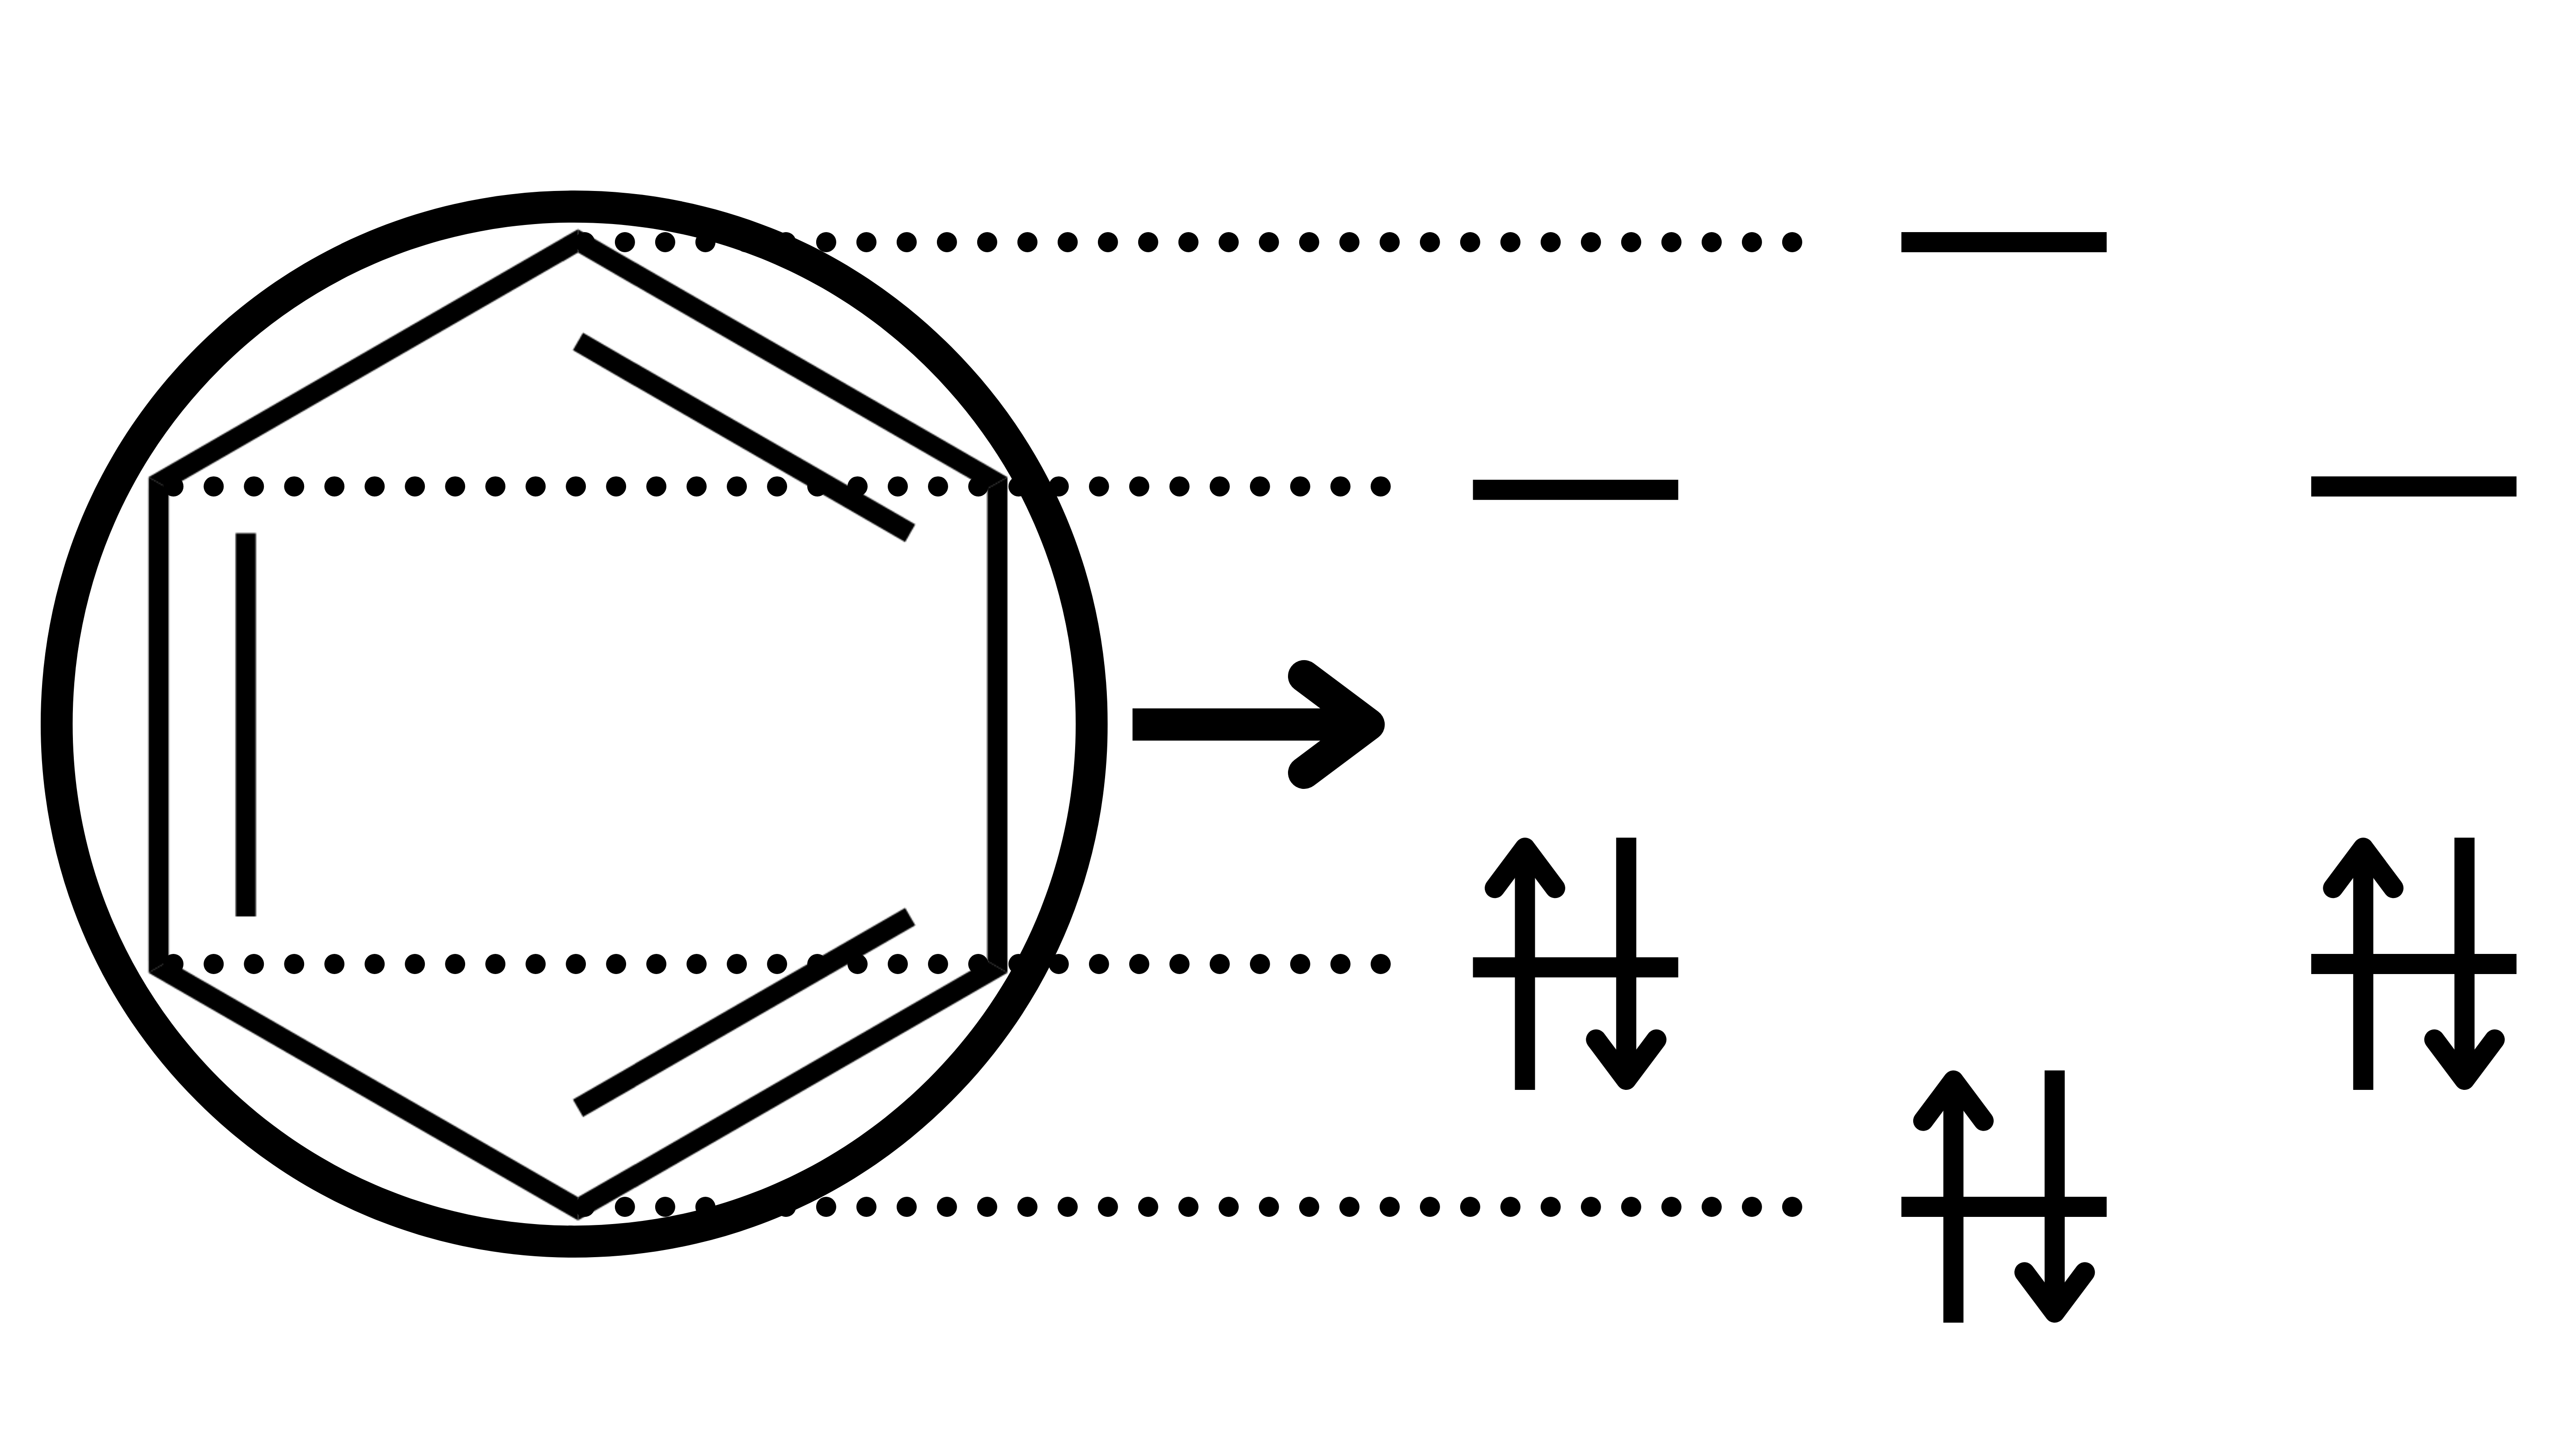
\includegraphics[width=0.60\textwidth]{images/figM.png}
	\end{center}
	\fonte{Autor(a).}
\end{figure}

%%% TODO : FROST DIAGRAM

Posteriormente, essa teoria foi estendida para tratar moléculas com heteroátomos (aqueles diferentes do carbono e hidrogênio)\autocite{Liwschitz1963}. Uma mudança ainda maior foi feita por Roald Hoffmann \autocite{Hoffmann1963}, que desenvolveu o método \gls{EHMO}, o qual inclui todos os elétrons da valência (inclusive elétrons $\sigma$) no cálculo das energias dos orbitais moleculares. Esse método é classificado como semiempírico, ou seja, utiliza dados experimentais para facilitar o processo de cálculo das integrais que acessam a interação elétron-elétron para contabilizar os efeitos de correlação eletrônica na estrutura molecular.

Como o objetivo do trabalho é desenvolver uma ferramenta rápida e eficiente para ser utilizada dentro no navegador de internet, tal método foi escolhido pelo seu baixo custo computacional de operação, devido às aproximações das matrizes Hamiltonianas pelo teorema de Koopman, cujas consequências fazem os valores de $H_{ii}$ serem substituídos pelas energias de ionização (leia o \autoref{ap:EHMO} para mais detalhes).

A metodologia de Hueckel estendido considera todos os elétrons da valência no cálculo, e baseia-se no princípio de que os orbitais moleculares são combinações de orbitais atômicos. Desse modo, os conjuntos de base mínimos utilizados para esse procedimento são os mesmos parâmetros empregados no \gls{YAeHMOP}\autocite{Avery2017}. 

\begin{figure}[htb]
    \vspace{2\baselineskip}
\begin{equation}
    \label{eq:LCAO}
    \tikzmarknode{lcao}{\highlight{red}{LCAO}} \Longrightarrow \psi_j = \sum_{r=1}^{N} c_{jr} \tikzmarknode{aos}{\highlight{blue}{$\phi_r$}}
\end{equation}
\begin{tikzpicture}[overlay,remember picture,>=stealth,nodes={align=left,inner ysep=1pt},<-]
    \path (lcao.north) ++ (-0.70,1.5em) node[anchor=south east,color=red!67] (scalep){\textit{combinação linear}};
    \draw [color=red!87](lcao.north) |- ([xshift=-0.70em,color=red]scalep.south west);
    
    \path (aos.south) ++ (-1,-1.5em) node[anchor=north east,color=blue!67] (scalep){\textit{orbitais atômicos (conjuntos de bases)}};
    \draw [color=blue!87](aos.south) |- ([xshift=-1.65em,color=blue]scalep.north west);
\end{tikzpicture}
\vspace{2\baselineskip}
\end{figure}

A energia do j-ésimo orbital é dada pela equação monoeletrônica de Schroedinger ($\hat{H}_{eff} \psi_j = \epsilon_j \psi_j$) usando um Hamiltoniano ($\hat{H}_{eff}$), que expressa a interação de um elétron com o restante da molécula.

\begin{figure}[htb]
    \vspace{3\baselineskip}
\begin{equation}
\label{eq:energy_j1}
        \epsilon_j = \frac{\tikzmarknode{hamil}{\highlight{blue}{$\displaystyle \langle \psi_j | \hat{H}_{eff} | \psi_j \rangle$}}}{\tikzmarknode{overlap}{\highlight{red}{$\displaystyle \langle \psi_j | \psi_j \rangle$}}}
\end{equation}
\begin{tikzpicture}[overlay,remember picture,>=stealth,nodes={align=left,inner ysep=1pt},<-]
    \path (hamil.north) ++ (-0.70,1.5em) node[anchor=south east,color=blue!67] (scalep){\textit{$\displaystyle \int \psi_j  \times \hat{H}_{eff} \times \psi_j d\tau$}};
    \draw [color=blue!87](hamil.north) |- ([xshift=-0.70em,color=blue]scalep.south west);
    
    \path (overlap.south) ++ (-1,-1.5em) node[anchor=north east,color=red!67] (scalep){\textit{$\displaystyle \int \psi_j \times \psi_j d\tau$}};
    \draw [color=red!87](overlap.south) |- ([xshift=-1.65em,color=red]scalep.north west);
\end{tikzpicture}
\vspace{2\baselineskip}
\end{figure}

A \autoref{eq:energy_j1} pode ser escrita como a \autoref{eq:energy_j} ao substituirmos a \autoref{eq:LCAO} na \autoref{eq:energy_j}.

\begin{equation}
\label{eq:energy_j}
    \epsilon_j = \frac{ \displaystyle \bigg{\langle} \sum_{r=1}^{N} c_{jr} \psi_r \bigg{|} \hat{H}_{eff} \bigg{|} \sum_{s=1}^{N} c_{js} \psi_s \bigg{\rangle}}{\displaystyle \bigg{\langle} \sum_{r=1}^{N} c_{jr} \psi_r \bigg{|} \sum_{s=1}^{N} c_{js} \psi_s \bigg{\rangle}}
\end{equation}

Generalizando a expressão da \autoref{eq:energy_j} para quaisquer orbitais moleculares, é omitido o índice $j$ (\autoref{eq:energy}).

\begin{equation}
\label{eq:energy}
    \epsilon = \frac{\displaystyle \sum_{r=1}^{N} \sum_{s=1}^{N} c^*_r c_s \langle \psi_r | \hat{H}_{eff} | \psi_s \rangle}{\displaystyle \sum_{r=1}^{N} \sum_{s=1}^{N} c^*_r c_s \langle \psi_r | \psi_s \rangle}
\end{equation}

Da \autoref{eq:energy} decorrem as integrais moleculares a serem calculadas (recomenda-se a leitura do \autoref{ap:HMO} e do \autoref{ap:EHMO} para mais detalhes):

\begin{itemize}
    \item $\displaystyle S_{rs} = \langle \psi_r | \psi_j \rangle$ é a integral de sobreposição. Como estamos trabalhando com orbitais normalizados, $S_{rr} = 1$;
    
    \item $\displaystyle H_{rr} = \langle \psi_r | \hat{H}_{eff} | \psi_r \rangle$ é a integral de Coulomb, aproximada pelo oposto do potencial de ionização (como é descrito no \autoref{ap:EHMO});
    
    \item $\displaystyle H_{rs} = \langle \psi_r | \hat{H}_{eff} | \psi_s \rangle$ é a integral de ressonância. Essa integral nos dá a energia de um elétron na região do espaço onde as funções $\phi_r$ e, $\phi_s$ sobrepõem-se. Os valores de $H_{rs}$ são computados pela \autoref{hamiltonian} (no \autoref{ap:EHMO}).
\end{itemize}

Substituindo então os elementos das integrais supracitadas na \autoref{eq:energy}, obtemos a \autoref{eq:energy_cont}.

\begin{equation}
\label{eq:energy_cont}
    \epsilon = \frac{\displaystyle \sum_{r=1}^{N} \sum_{s=1}^{N} c^*_r c_s H_{rs}}{\displaystyle \sum_{r=1}^{N} \sum_{s=1}^{N} c^*_r c_s S_{rs}}
\end{equation}

\subsection{Integral de sobreposição}\label{sec:overlap}

No Método de Hueckel Estendido, as integrais de sobreposição são calculadas utilizando orbitais atômicos de Slater (representado por coordenadas esféricas na \autoref{stos}), pois seus resultados são mais acurados (mesmo que não sejam solução exata), principalmente pelo fato de reproduzirem mais precisamente a região do cúspide e o decaimento orbital. Essa aproximação é feita porque a descrição matemática dos orbitais atômicos não pode ser exatamente conhecida, mas aproximada pela forma dos orbitais dos sistemas hidrogeniônicos, uma vez que o problema torna-se intratável analiticamente para qualquer sistema multieletrônico. Desse modo, os conjuntos de bases são obtidos pelas regras de Slater\autocite{Slater1930, Lu2006}.

\begin{figure}[htb]
    \vspace{3\baselineskip}
\begin{equation}
\label{stos}
        \tikzmarknode{sto}{\highlight{blue}{$\chi_{nlm}(\zeta, r)$}} = \tikzmarknode{norm}{\highlight{gray}{$N$}} r^{n-1} e^{-\zeta r} \tikzmarknode{harmonic}{\highlight{red}{$Y_l^m (\theta, \Phi)$}}
\end{equation}
\begin{tikzpicture}[overlay,remember picture,>=stealth,nodes={align=left,inner ysep=1pt},<-]
    \path (sto.south) ++ (-0.70,-1.5em) node[anchor=north east,color=blue!67] (scalep){\textit{Slater Type Orbital}};
    \draw [color=blue!87](sto.south) |- ([xshift=-0.70em,color=blue]scalep.north west);
    
    \path (norm.south) ++ (0.70,-1.5em) node[anchor=north west,color=gray!67] (scalep){\textit{$\displaystyle \bigg{[} \frac{(2 \zeta)^{n-1}}{(2n)!} \bigg{]}^{1/2}$}};
    \draw [color=gray!87](norm.south) |- ([xshift=0.70em,color=gray]scalep.north east);
    
    \path (harmonic.north) ++ (-0.70,1.5em) node[anchor=south east,color=red!67] (scalep){\textit{função angular}};
    \draw [color=red!87](harmonic.north) |- ([xshift=-0.70em,color=red]scalep.south west);

\end{tikzpicture}
\vspace{2\baselineskip}
\end{figure}

\noindent onde:

\begin{equation}
    \textcolor{red!67}{i^{m + |m|}\bigg{[}\displaystyle \frac{(2l+1)(l+|m|)!}{2(l + |m|)!}\bigg{]}^{1/2} P^m_l (cos \; \theta) \phi_m(\Phi)}
\end{equation}

Avaliando a \autoref{stos}, $N$ representa a constante de normalização, $r^{n-1}e^{-\zeta r}$ é a parte radial da função (onde $r$ é a distância entre o elétron e o núcleo do átomo e $\zeta$ é uma constante de proteção relacionada à carga efetiva do núcleo, sendo a carga nuclear parcialmente protegida por elétrons), e $Y_l^m (\theta, \Phi)$ representa a parte angular, onde os esféricos harmônicos normalizados são relacionados com polinômios de Legendre, definido pela \autoref{legendre}, e $\phi_m (\Phi)$ representa as funções ortonormais.

\begin{figure}[htb]
\begin{equation}
    \phi_m (\Phi) = (2\pi)^{-1/2} e^{im\Phi}
\end{equation}
\end{figure}

\begin{figure}[htb]
    \vspace{3\baselineskip}
\begin{equation}
\label{legendre}
    P^m_l(x) = (1 - x^2)^{m/2} \sum_{u=0}^{l - m} \tikzmarknode{c}{\highlight{blue}{$C_{lmu}$}} x^u
\end{equation}
\begin{tikzpicture}[overlay,remember picture,>=stealth,nodes={align=left,inner ysep=1pt},<-]
    \path (c.north) ++ (-0.50,1.5em) node[anchor=south east,color=blue!67] (scalep){\textit{$C_{lmu} = \displaystyle \frac{(-1)^{(l-m-u)/2}[1 + (-1)^{(l - m - u)}](l + m + u)!}{2^{l + 1}([l - m - u]/2)!([l + m + u]/2)!}$}};
    \draw [color=blue!87](c.north) |- ([xshift=-0.20em,color=blue]scalep.south west);
\end{tikzpicture}
\end{figure}

De maneira geral, pode-se definir, portanto, as integrais de sobreposição \autocite{Hoggan2011}
definida por coordenadas esféricas.

\begin{equation}
\label{overlap}
    S^{n_2 l_2 m_2}_{n_1 l_1 m_1} (\zeta_1; \zeta_2; \textbf{\textit{R}} ) = \int [\chi_{n_1 l_1 m_1} (\zeta_1, \textbf{\textit{r}})]^* \chi_{n_2 l_2 m_2} (\zeta_2, \textbf{\textit{r - R}})
\end{equation}

A expressão da \autoref{overlap} pode ser aproximada a uma expressão analítica por uma série de somatórios finitos ponderados por coeficientes binomiais, podendo então serem mais facilmente computadas e calculadas.

\begin{figure}[htb]
    \vspace{4\baselineskip}
\begin{equation}
\label{analitica}
\begin{split}
    S^{n_2 l_2 m_2}_{n_1 l_1 m_1} (\zeta_1; \zeta_2; \textbf{\textit{R}} ) = N N' (R/2)^{n_1 + n_2 + 1} \tikzmarknode{auxiliary}{\highlight{blue}{$D(l_1, l_2, m)$}}  \\[0.35cm] \sum_{u=0}^{l_1 - m} \sum_{v=0}^{l_2 - m} \sum_{p=0}^{n_1 - m - u} \sum_{p'=0}^{n_2 - m - v} \sum_{q=0}^{m} \sum_{q'=0}^{m} \sum_{t=0}^{u}  \sum_{t'=0}^{v} (-1)^{n_1 - m - u} C_{l_1 m u} C_{l_2 m v} \\[0.35cm] F_p (n_1 - m - u) F_{p'} (n_2 - m - v)
    F_q (m) F_{q'} (m) F_t (u) F_{t'} (v) A_i (\alpha) B_j (\beta) 
\end{split}
\begin{tikzpicture}[overlay,remember picture,>=stealth,nodes={align=left,inner ysep=1pt},<-]
    \path (auxiliary.north) ++ (-0.50,1.5em) node[anchor=south east,color=blue!67] (scalep){\textit{$D(l_1, l_2, m) = \displaystyle \sqrt{\frac{(2l_1 + 1)(2l_2 + 1)(l_1 - m)!(l_2 - m)!}{4(l_1 + m)!(l_1 + m)!}}$}};
    \draw [color=blue!87](auxiliary.north) |- ([xshift=-0.20em,color=blue]scalep.south west);
\end{tikzpicture}
\end{equation}
\end{figure}

Nessa expressão (\autoref{analitica}), $A_i (\alpha)$ e $B_j (\beta)$ são funções auxiliares, $\alpha = R(\zeta_1 + \zeta_2)/2$, $\beta = R(\zeta_1 - \zeta_2)/2$ e $F_n(m)$ são os coeficientes binomiais \autocite{Mekelleche1997} e os termos $i$ e $j$ estão descritos na \autoref{termos}.

\begin{align}
\label{termos}
    i = n_1 + n_2 - 2m - p - p' + 2q - t - t' \\
    j = p + p' + 2m - 2q' + u + v - t - t'
\end{align}

%\section{Otimização de geometria}

%Predizer o arranjo mais estável dos átomos em uma molécula é uma das mais importantes tarefas na %química quântica computacional. Essencialmente, este é um problema de otimização onde a energia total %da molécula é minimizada com relação às posições dos núcleos atômicos. A geometria molecular obtida %desse cálculo é, dessa forma, um ponto de partida para inúmeras simulações de propriedades %moleculares. Se a geometria não é acurada, então quaisquer cálculos que derivam dele também podem ser %espúrios.

%Uma vez que os núcleos são muito mais pesados do que os elétrons, nós podemos tratá-los como %partículas pontuais associadas às suas respectivas posições. A partir disso, é possível afirmar que a %energia da molécula $E(x)$ depende das coordenadas nucleares $x$, as quais definem a energia de %superfície potencial. Resolver, portanto, o problema estacionário $\nabla_x E(x)$, corresponde à %otimização das coordenadas nucleares, e a partir delas é possível determinar a energia de equilíbrio %da molécula.

%No trabalho em questão, foi utilizado um método genérico (variacional) para encontrar a estrutura %situada na região de mínima energia. A ideia central desse algoritmo é considerar explicitamente o %Hamiltoniano $H(x)$ como uma observável parametrizada, que depende das coordenadas nucleares $x$. O %objetivo desse procedimento é encontrar o mínimo global da função de custo global $g(\theta, x) = < %\Psi(\theta) | H(x) | \Psi(\theta) >$.



\section{Teoria de grafos}

Ao acessar a interface gráfica, será possível ao usuário fornecer um arquivo de extensão \textit{.xyz}, contendo as informações em coordenadas cartesianas da estrutura a ser analisada (\autoref{workflow}). O sistema de interesse será processado computacionalmente e transformado em um grafo $G$, que corresponde a uma coleção de vértices (pontos) chamados genericamente de $V$ e arestas (linhas) denotadas por $E$. Formalmente um grafo simples $G$ é definido como um par ordenado $(V(G), E(G))$, o qual consiste de um conjunto $V(G)$ de vértices $V$ não vazio e um conjunto de arestas $E(G) = E$ contendo pares não ordenados de elementos distintos de V, uma vez que cada elemento de $E(G)$ é uma linha que conecta dois pontos de $V(G)$. Para maiores detalhes sobre a teoria de grafos, acesse o \autoref{ap:graph}.

\begin{figure}[htb]
	\caption{\label{fig:M2} Exemplo ilustrativo de um grafo cíclico não direcionado. Os pontos em azul representam os seis vértices que se conectam através das linhas pretas correspondentes às arestas. O equivalente à esquerda é um anel benzênico de Kekulé, com seis átomos de carbono ocupando os nodos de um ciclo hexagonal.}
	\begin{center}
		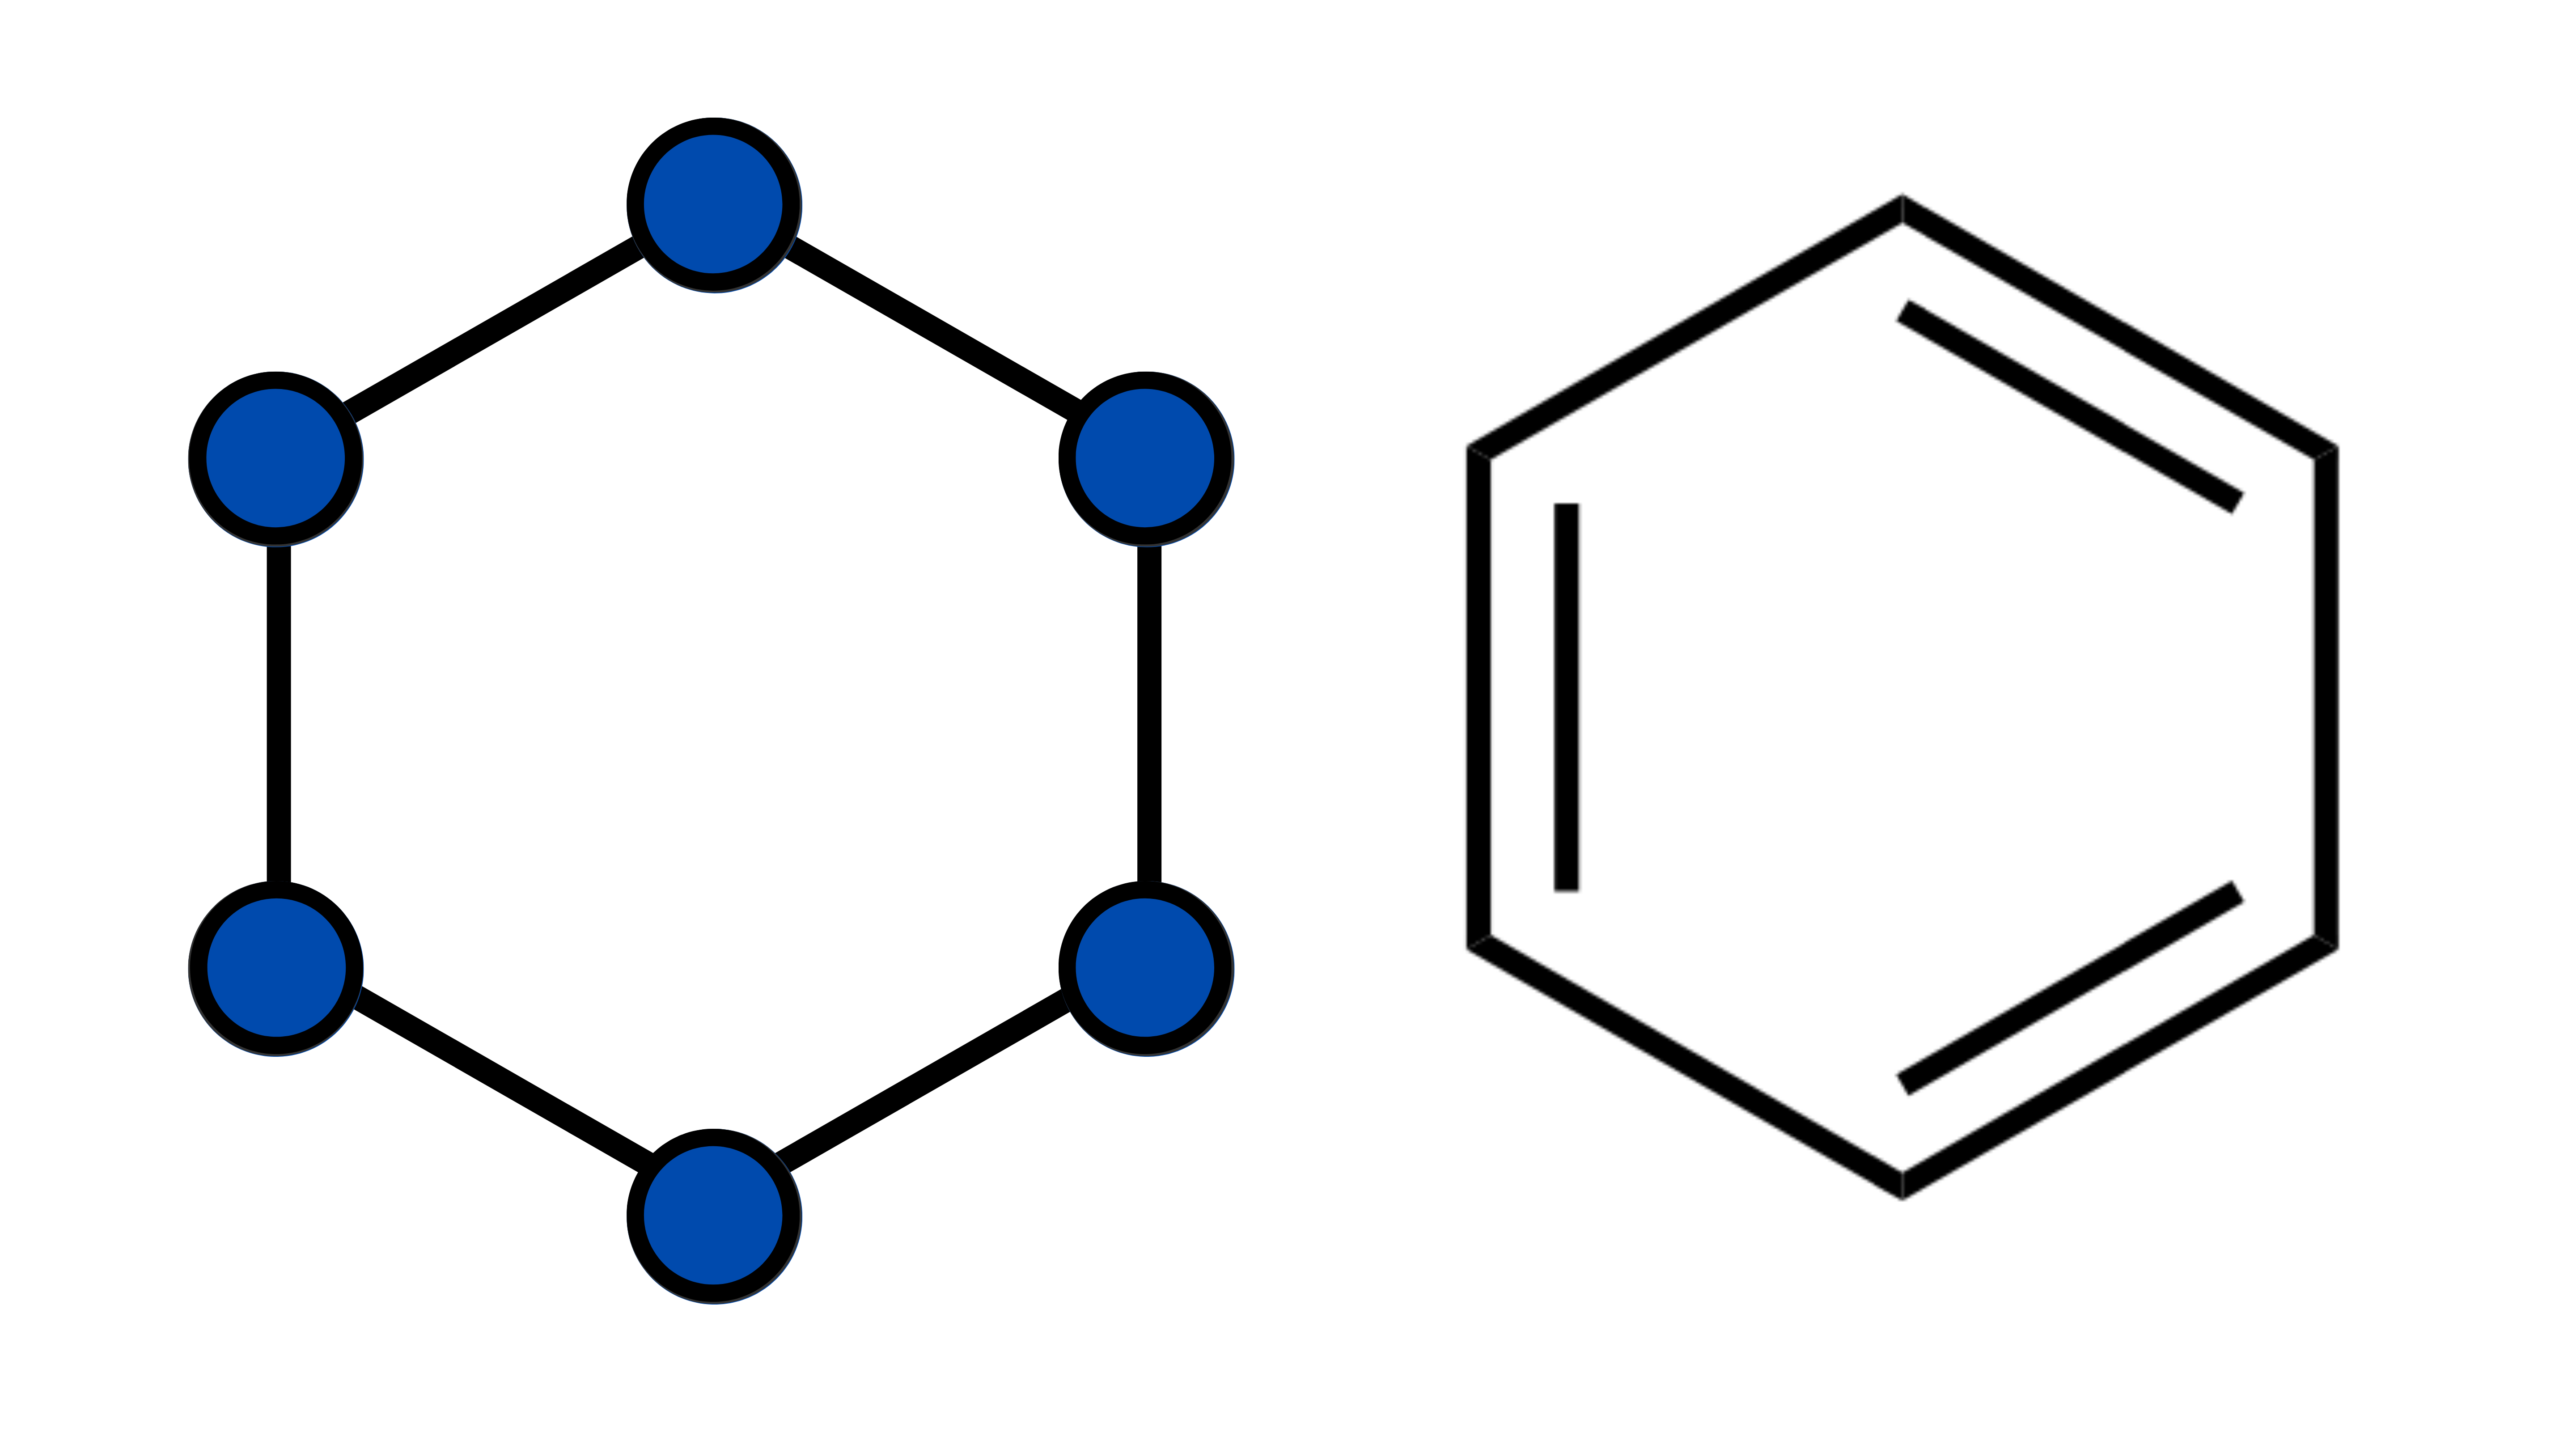
\includegraphics[width=0.55\textwidth]{images/grafo(2).png}
	\end{center}
	\fonte{Autor(a).}
\end{figure}

\begin{figure}[htb]
\caption{\label{fig:graphEnumerated}Representação do grafo mostrado na \autoref{fig:M2} com nodos enumerados sequencialmente de 1-6.}
	\begin{center}
		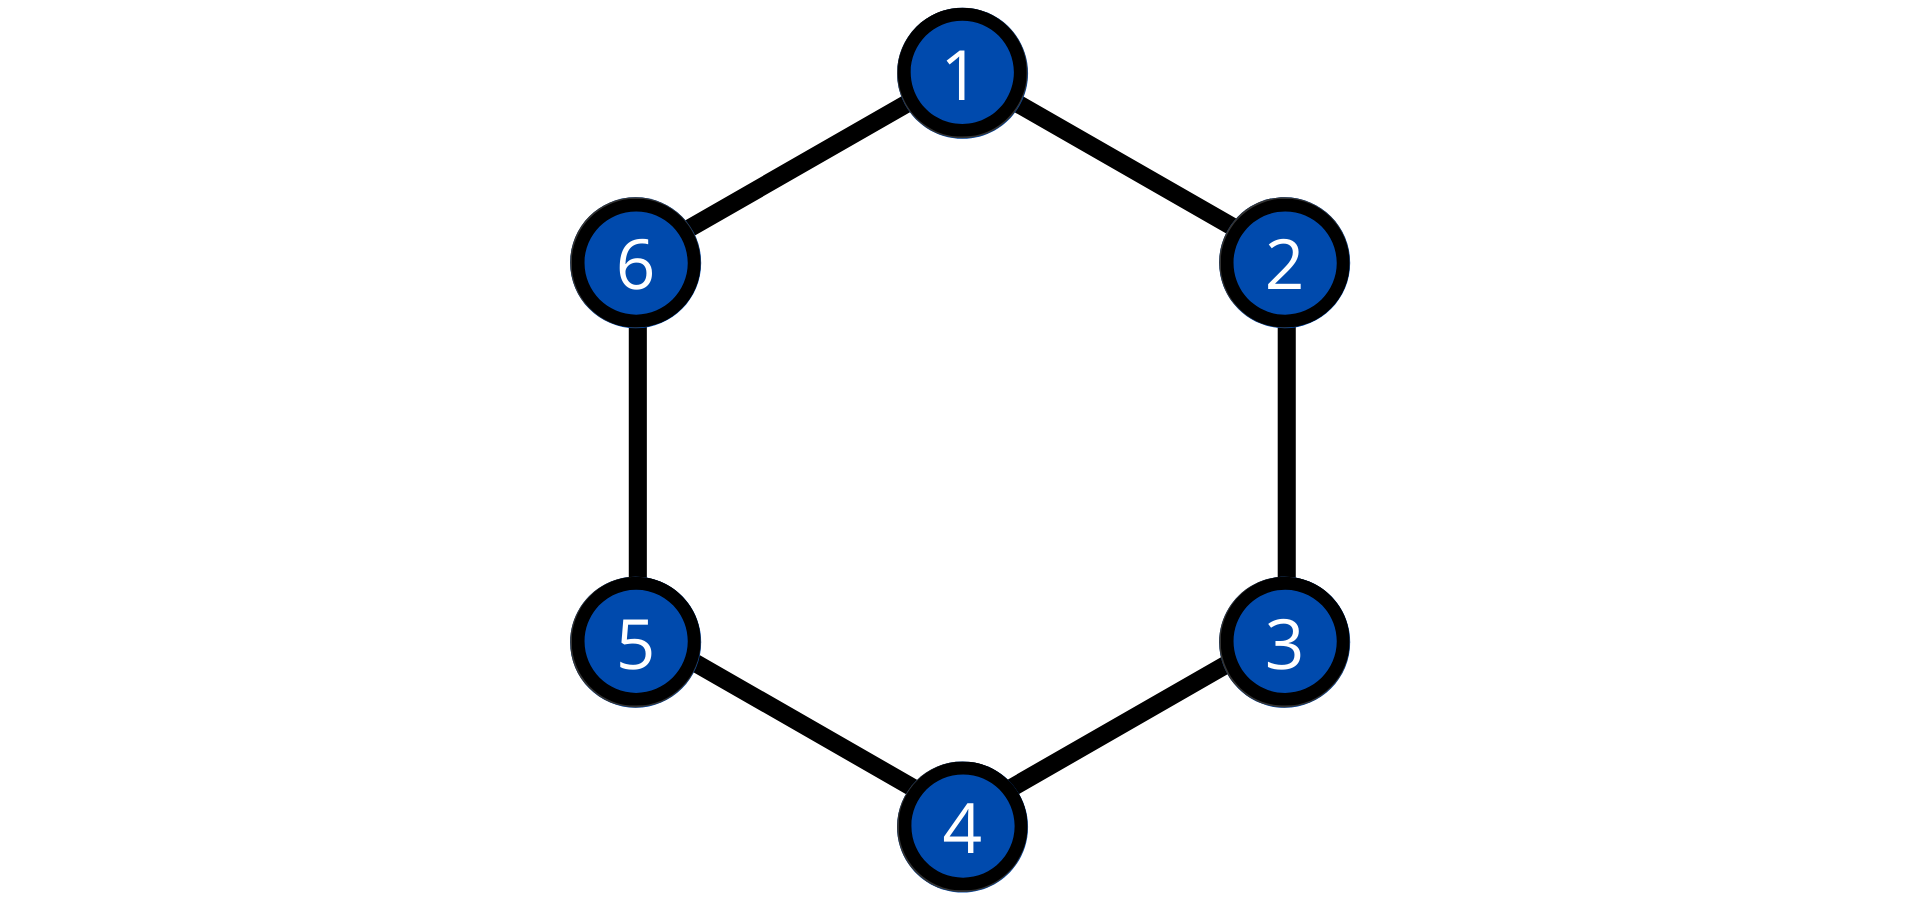
\includegraphics[width=0.55\textwidth]{images/graphEnumerated.png}
	\end{center}
	\fonte{Autor(a)}
\end{figure}

Desse modo, transpõe-se a representação apresentada na \autoref{fig:M2} para as estruturas químicas de interesse, uma vez que os átomos podem ser considerados os análogos químicos dos vértices, e as ligações, das arestas. Enumerando-se sequencialmente os nodos do grafo derivado do benzeno como na \autoref{fig:graphEnumerated}, é possível então verificar computacionalmente onde esses pontos estão localizados. Ao identificar a estrutura como um grafo, é mais fácil construir a matriz do determinante secular da teoria \gls{EHMO} (veja a discussão desse resultado na \autoref{sec:benzene}). 

O \gls{DFS}\autocite{Knuth1997-jf, Goodrich2001-pd} é um algoritmo recursivo que perpassa todos os vértices de um grafo ou de uma árvore de dados através do conceito de \textit{backtracing} (retorno). Ou seja, ele começa em um nodo raiz definido arbitrariamente e a partir dele explora suas adjacências através da expansão da árvore de busca, aprofundando-se até que o alvo da busca seja encontrado ou até que ele se depare com um nó que não possui adjacências (nodo folha). Então a busca retrocede (\textit{backtrack}) e começa no próximo nó. Numa implementação não-recursiva, todos os nós expandidos recentemente são adicionados a uma pilha, para realizar a exploração (Algoritmo \ref{alg:1}, \autoref{fig:DFS}).

\begin{figure}[htb]
\caption{\label{fig:DFS} Representação esquemática do algoritmo DFS (Algoritmo \ref{alg:1}). Todos os nodos adjacentes são visitados até que sejam marcados como visitados (cinza). O ciclo é encontrado quando o último nodo é igual ao nodo raiz.}
	\begin{center}
		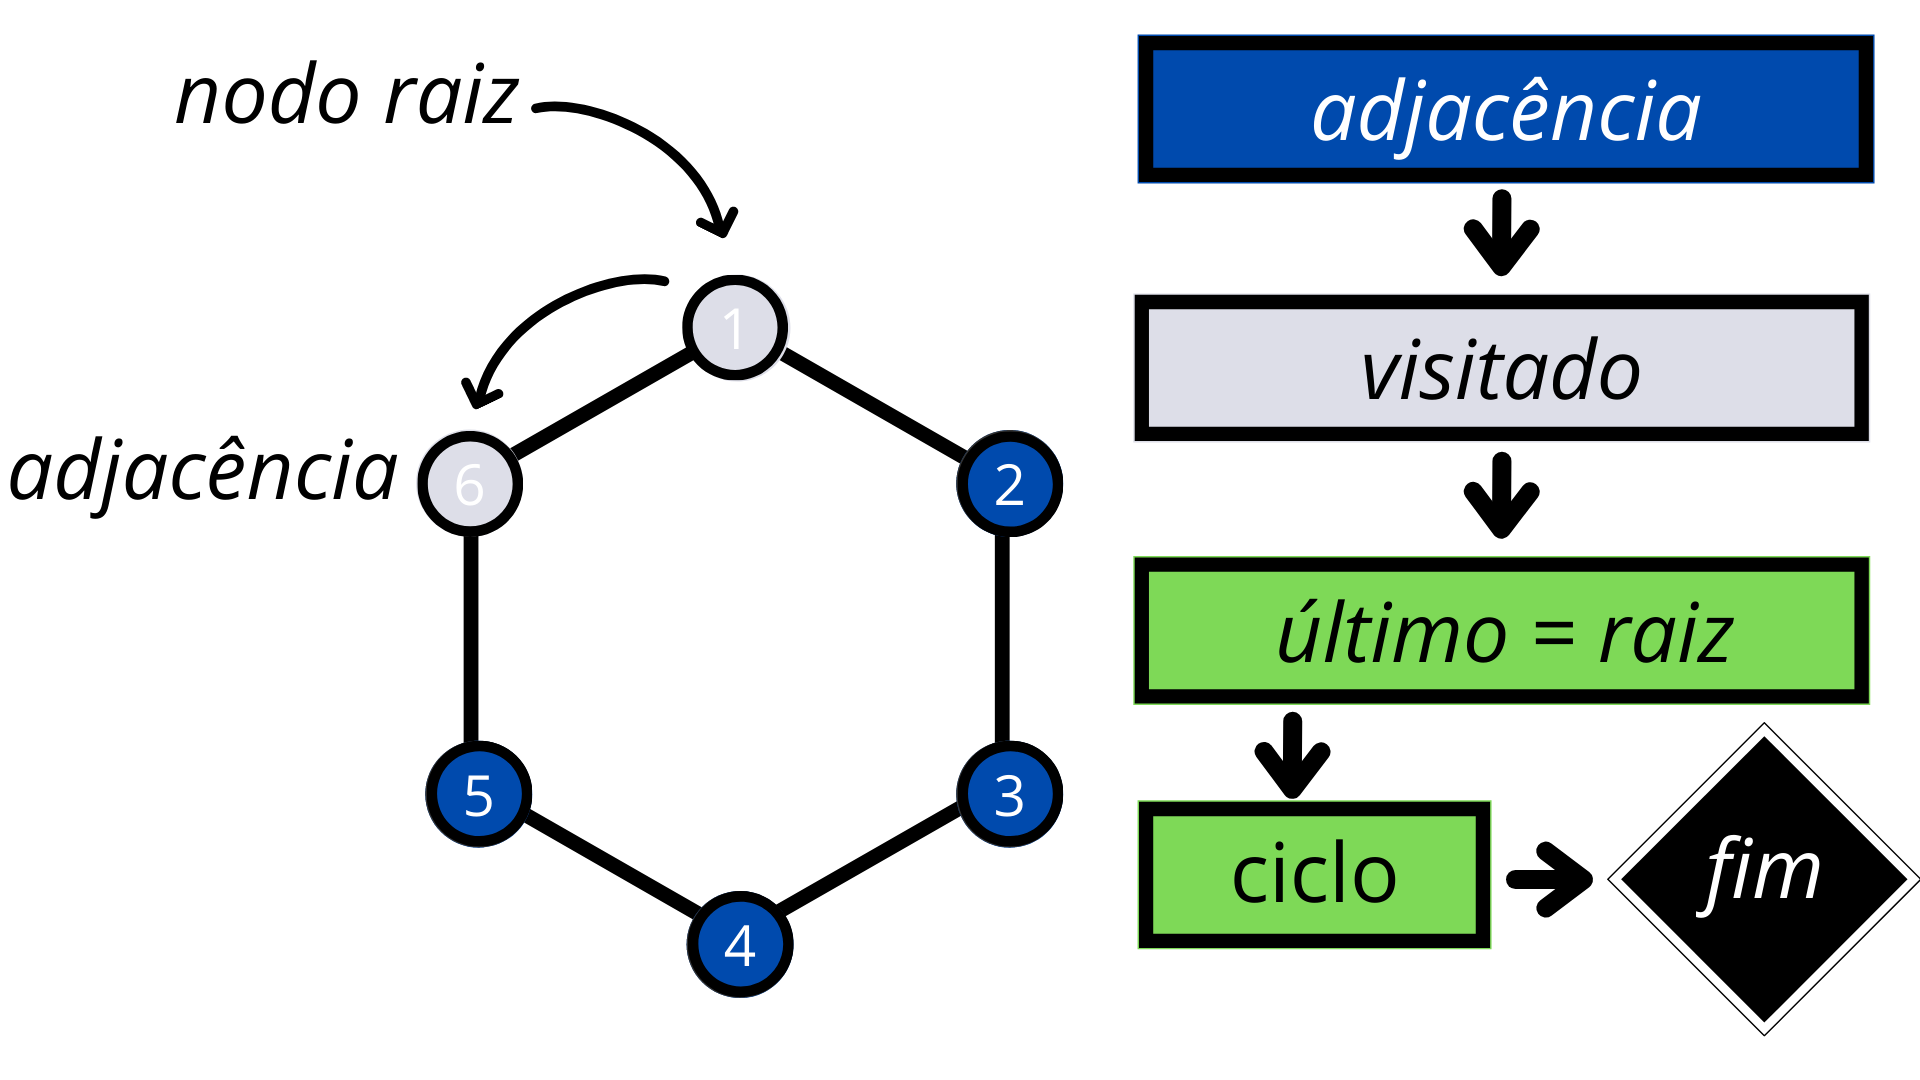
\includegraphics[width=0.65\textwidth]{images/DFS.png}
	\end{center}
	\fonte{Autor(a)}
\end{figure}

\SetKwComment{Comment}{/* }{ */}

\begin{algorithm}
\caption{Detecção de ciclos em grafos via DFS}\label{alg:1}
\LinesNumbered
\KwData{vértice geral $v_n$ }
\KwResult{$true$ se o ciclo é encontrado}
\SetKwFunction{FMain}{detectcycle}

  \SetKwProg{Pn}{Function}{}{}
  \Pn{\FMain{$v_n$}}{$mark(v_n, visited\;)$\;
        \For{$ v_{n'} \in \; neighbors(v_n) $}{
        \eIf{$mark(v_n) == \; visited$}
        {\If{$v_n ==v_{n'}$ \textbf{or} $v_n \; != \; parent(v_{n'})$}{\textbf{return} $true$ \;}}
        {\If{$detectcycle(v_{n'})$}{\textbf{return $true$} \;}}
    }
    }
\end{algorithm}

Ao identificar os ciclos a partir do algoritmo \gls{DFS}, é possível classificar os ciclos, análogos aos anéis aromáticos, e calcular os índices geométricos (para uma descrição do formalismo dos índices geométricos, veja a \autoref{sec:HOMA}) referente a cada um dos sextetos das estruturas policíclicas (veja um exemplo dessa aplicação na \autoref{sec:policicle}). 

\section{Tratamento de resíduos}

Como o trabalho em questão é teórico, foram utilizadas ferramentas computacionais dentro do Grupo de Estrutura Eletrônica Molecular (GEEM) da Universidade Federal de Santa Catarina (UFSC) para o desenvolvimento do mesmo. Desse modo, em caso de geração de lixo eletrônico, o descarte foi feito de forma apropriada junto às estações de coleta seletiva específicas, conhecidas como Ecopontos.